\subsection{Jupiter}
\label{algo:jupiter}

\emph{Jupiter} is a multi-user, multimedia virtual world intended to support long-term remote collaboration. In particular, it supports shared documents, shared tools, and, optionally, live audio/video communication. It is basically a collaborative windowing toolkit. The low-level communication facilities (operational transformation) are described in \cite{jupiter95}.

\emph{Jupiter}'s algorithm is derived from \emph{dOPT}. The centralized architecture and thus the reduction of point-to-point connections allows them to simplify the \emph{dOPT} algorithm. Several point-to-point connections are used to build a tree-structured $n$-site algorithm.

\emph{Jupiter} solves the \emph{dOPT} puzzle. It uses a two dimensional state space instead of a linear history buffer (request log) to save operations. It transforms saved messages against conflicting incoming messages. Unfortunately, simply transforming saved messages does not work for the $n$-way case, since the next message can come from a third site that is in an inconvenient message state. See \emph{adOPTed} \ref{algo:adopted} for a solution to the $n$-way case.


\subsubsection{Details}

The general tool for handling conflicting (concurrent) messages is the transformation function, called \emph{xform} in \cite{jupiter95}.

$$ xform(c,s)={c',s'} $$

It takes a message $c$ from the client and a message $s$ from the server and returns two transformed messages $c'$ and $s'$. The messages $c'$ and $s'$ have the property that if the client applies $c$ followed by $s'$, and the server applies $s$ followed by $c'$, both client and server wind up in the same final state. The \emph{xform} function is basically a combined inclusion transformation (IT) function that returns the result of both $IT(c,s)$ and $IT(s,c)$.

It is helpful to show the two dimensional state space that both client and server pass through as they process messages (see figure \ref{jupiter:statespace1}). Each state is labelled with the number of messages from the client and server that have been processed to that point. For instance if the client is in the state $(2,3)$, it has generated and processed two messages of its own, and has received and processed three from the server. The client and server messages are displayed on different axis in the state space. 

If there is a conflict, the paths will diverge, as shown in figure \ref{jupiter:statespace1}. The client and server moved to the state $(1,1)$ together by first processing a client message, and then a server message. At that point, the client and server processed different messages (concurrently), moving to state $(2,1)$ and $(1,2)$ respecitvely. They each received and processed the other's message using the transformation function to move to state $(2,2)$. Then the server generated another message, sending it to the client and both were in state $(2,3)$.

\begin{figure}[H]
  \centering
  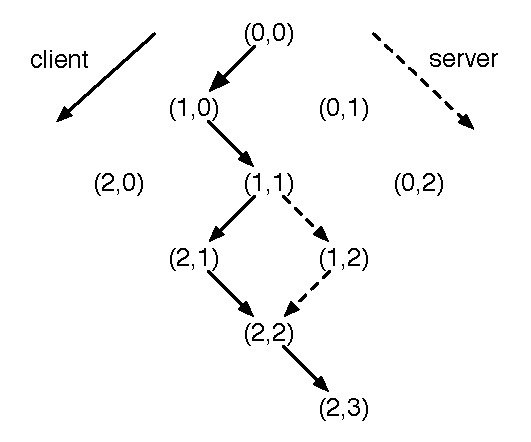
\includegraphics[width=3in,height=2.45in]{../../images/jupiter2.eps}
  \caption{Two dimensional state space example}
  \label{jupiter:statespace1}
\end{figure}

The algorithm labels each message with the state the sender was in just before the message was generated (state vector). The recipient uses these labels to detect conflicts. Two concurrent messages have to be transformed, but they can only be transformed directly when they were generated from the same state of the document. 

If client and server diverge more than one step, the transformation function cannot be applied directly. Consider figure \ref{jupiter:statespace2}. The client has executed $c$ and receives the conflicting message $s1$ from the server. It uses the transformation function to compute $s1'$ to get to the state $(1,1)$. The server then generates $s2$ from the state $(0,1)$, indicating that it still has not processed $c$. What should the client do now? It cannot use the transformation function directly because $c$ and $s2$ were not generated from the same document state.

\begin{figure}[H]
 \centering
 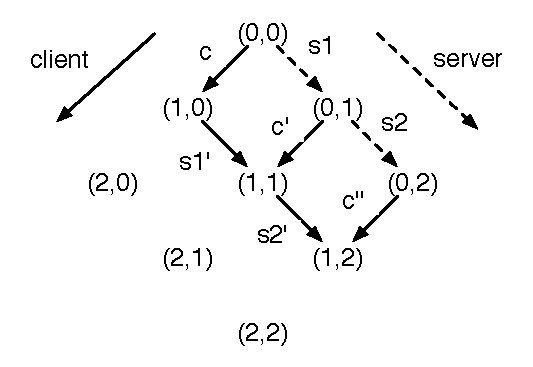
\includegraphics[width=3in,height=2in]{../../images/jupiter.eps}
 \caption{Conflicting messages}
 \label{jupiter:statespace2}
\end{figure}

The solution to this situation is as follows. When the client computes $s1'$ it must also remember $c'$. This represents a hypothetical message that the client could have generated to move from the state $(0,1)$ to $(1,1)$. When $s2$ arrives, the client can use $c'$ to compute $c''$. It executes $s2'$ to get to the state $(1,2)$. If the server has processed the client's message, it will be in the state $(1,2)$ as well. If not, its next message will originate from $(0,3)$, so the client saves $c''$ just in case.

The algorithm guarantees that, no matter how far the client and server diverge in state space, when they do reach the same state, they will have identical states (so convergence is achieved).


\subsubsection{Properties}
\begin{itemize}
 \item uses state vectors to determine causality relations
 \item uses multiple 2-way synchronization protocols to create a n-way protocol
 \item free of TP2
 \item very simple algorithm
 \item two dimensional state space graph
 \item architecture: replicated, unicast
\end{itemize}
